\documentclass{scrartcl}
\usepackage{style}
% version
\newcommand{\versionmajor}{0}
\newcommand{\versionminor}{1}
\newcommand{\versionpatch}{0}
\newcommand{\version}{\versionmajor.\versionminor.\versionpatch}

\title{\LARGE
    Final Report Template
}

\subtitle{(v. \version)}

% Consider watching:
% https://www.youtube.com/watch?v=ihxSUsJB_14
% https://www.youtube.com/watch?v=XTFWaV55uDo

\author{
    Author 1 \\ \emailaddr{author1@email.it}
    \and 
    Author 2 \\ \emailaddr{author2@gmail.com} 
    \and 
    Author 3 \\ \emailaddr{author3@unibo.it}
}

\date{\today}

\begin{document}

\maketitle

\begin{abstract}
    Up to $\sim$2000 characters briefly describing the project (i.e. its goals and results).
\end{abstract}

\section{Goal/s of the project}

Detailed description of the project goal/s.
%
Use case diagrams, examples, or Q/A simulations are welcome.

\subsection{Usage scenarios}

Informal description of the ways users are expected to interact with your project.
%
It should describe \emph{how} and \emph{why} a user use / interact with the system.

\subsection{Definition of done}

\begin{itemize}
    \item Which kind of \emph{artefacts} will be delivered?
    %
    \item How will the system \emph{functionality} be tested?
    %
\end{itemize}

\section{Background and link to the theory}
%
(To be written at the end)
%
\begin{itemize}
    \item Relevant architectural styles (the ones mentioned in \Cref{sec:requirements})
    %
    \item Relevant interaction patterns (the ones mentioned in \Cref{sec:requirements}) 
    %
    \item Relevant software frameworks (the ones mentioned in \Cref{sec:requirements,sec:design}) 
\end{itemize}

\section{Requirements Analysis}
\label{sec:requirements}

\subsection{Requirements list}
%
\begin{itemize}
    \item Functional
    %
    \item Non functional
    %
\end{itemize}
%

\subsection{Top-down analysis}
%
\begin{itemize}
    \item What architectural style / interaction pattern / software framework are better suited to develop the project
    %
    \item \dots and why w.r.t. requirements
    %
\end{itemize}
%

\section{Design}
\label{sec:design}

This is where the logical / abstract contribution of the project is presented.
%
Always remember to report \textbf{why} a particular design has been chosen.
%
Keep the discussion \emph{technology-free} as much as possible.
%
Reporting wrong design choices which has been evaluated during the design phase is welcome too.

\subsection{Structure (domain entities)}

Which entities need to by modelled to reflect the domain?
%
UML class diagram here with domain entities and possibly messages being exchanged

\subsection{Interaction}

How should entities interact with each others?
%
UML activity / sequence diagram and protocols definitions.

\subsection{Behaviour}

How should each entity behave?
%
UML State diagram.

\subsection{Architecture}

How are software pieces organised into software modules?
%
UML component / package / deployment diagrams, data-flow among components, web API description.

\subsection{Corner cases}

\begin{itemize}
    \item Faults detection
    %
    \item Recover strategies
    %
    \item Error messages
    %
    \item Graceful shutdown
\end{itemize}

\section{Salient implementation details}

Anything potentially interesting / non-trivial and technologies adopted to match the design.
%
This section is expected to be short in case some documentation (e.g. Javadoc or Swagger Spec) has been produced for the software artefacts.
%
This this case, the produced documentation should be referenced here.

\section{Validation}

Choose a criterion for the evaluation of the produced software and \textbf{its compliance to the requirements above}.
%
Description of automated (and manual) tests and their rationale.
%
In case of a test-driven development, describe tests here and possibly report the amount of passing tests, the total amount of tests and, possibly, the test coverage.

\section{Deployment Instructions}

Explain here how to install and launch the produced software artefacts.
%
Assume the software must be installed on a totally virgin environment.
%
So, report \textbf{any} configuration step.
%
Gradle and Docker may be useful here to ensure the deployment and launch processes to be easy.

\section{Usage Examples}

Show how to use the produced software artefacts.
%
Ideally, there should be at least one example for each scenario proposed above.

\section{Conclusions}

Recap what you did.

\subsection{Future Works}

Recap what you did \emph{not}

\subsection{What did we learned}

Recap what did you learned.

\section*{Stylistic Notes}

Use a uniform style, especially when writing formal stuff: $X$, X, $\mathbf{X}$, $\mathcal{X}$, \texttt{X} are all different symbols possibly referring to different entities. 

This is a very short paragraph.

This is a longer paragraph (notice the blank line in the code).
It composed by several sentences.
%
You're invited to use comments within \texttt{.tex} source files to separate sentences composing the same paragraph.

Paragraph should be logically atomic: a subordinate sentence from one paragraph should always refer to another sentence from within the same paragraph.

The first line of a paragraph is usually indented.
%
This is intended: it is the way \LaTeX{} lets the reader know a new paragraph is beginning.

\begin{figure} % DO NOT write any positional hint (e.g. [h] or [t] here!
    \centering
    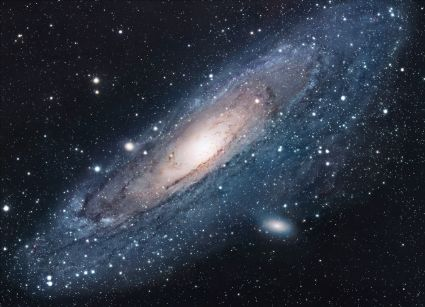
\includegraphics[width=0.5\linewidth]{figures/universe.jpg}
    \caption{Some floating image}
    \label{fig:image} 
\end{figure}

Let \LaTeX{} decide where to put figures (or tables, or listings), label them and reference the labels instead of say things like ``in the following image...''.
%
Consider for instance the case of \cref{fig:image}.

Use the \href{https://en.wikibooks.org/wiki/LaTeX/Source_Code_Listings}{\texttt{listing}} package for inserting scripts into the \LaTeX{} source.
%
Consider for instance \cref{lst:snippet}.

% have a look to macros in code-listings.sty
\javaimport[
    caption={Some Java listing},
    label={lst:snippet}
]{listings/HelloWorld.java}

\nocite{*} % Includes all references from the `references.bib` file
\bibliographystyle{plain}
\bibliography{references}

\end{document}
